\documentclass[twocolumn]{article}
\usepackage{graphics}
\usepackage{graphicx}
\usepackage[utf8]{inputenc}
\usepackage{hyperref}
\usepackage{natbib}
\usepackage{amsmath}
\usepackage{algorithm2e}
\usepackage[inkscapeformat=png]{svg}

% \usepackage{themeKonstanz}
% \usepackage{themeKonstanzXelatexAddOn}

\newcommand{\aetitle}{Comparison of an approximation, heuristic and integer-linear program for the max-cut problem on unweighted, undirected graphs} % Title of the report
\newcommand{\studentOne}{Jakob Sanowski} % Name 1
\newcommand{\studentTwo}{} % Name 2


\begin{document}

\twocolumn[{\begin{small}
\begin{minipage}{0.5 \linewidth}
  Algorithm Engineering\\
  WS 21/22
\end{minipage}
\begin{minipage}{0.5\linewidth}
  \begin{flushright}
    \studentOne\\
    \studentTwo
  \end{flushright}
\end{minipage}
\end{small}}
{\begin{center}
\begin{sffamily}\Large\bfseries \aetitle \end{sffamily}
\end{center}}
\vskip 3em]

\begin{abstract}
  I implemented and compared a heuristic, a approximation algorithm and an Integer-Linear-Program formulation
  for the maximum-cut problem on graphs. First I explain the algorithms and show their theoretical guarantees.
  The implementations are tested and evaluated on 60 graphs of different size. The results show the basic 
  heuristic being the fastest while the approximation algorithm achieves the higher quality results.
  Solving maximum-cut with an Integer-Linear-Program solver is only really feasible on sparse graphs.
\end{abstract}


\section{Introduction}
% The Introduction is meant to lead the reader into the task at hand. State the motivation and purpose of your project, and name the achieved goals.
The max-cut problem is a widely known problem on graphs. 
It is known to be NP-Hard but there exist a wide variety of approximation algorithms and heuristics for it.
In this report we will look at a simple heuristic and approximation algorithm as well take a look at an
Integer-Linear-Program formulation for it [\cite{algorithms}].
We will focus on the performance and quality of the result on differently sized graphs.
The heuristic and the approximation algorithm have in common, that they both achieve a 0.5-approximation.
This report is structured as follow. In Section \ref{sct:pre} we will look at the underlying ideas of
the algorithm. Section \ref{sct:impl} will provide details about the implementation and ideas on how
to improve the algorithms.
Following that, in Section \ref{sct:res} the setup of the experiments is outlined and the results are presented.
Finally, Section \ref{sct:dis}, we will discuss the findings of this report and draw further conclusions.


\section{Preliminaries}
\label{sct:pre}
% The preliminaries provide the reader with necessary background information. In this section the basic algorithms and the ideas behind them are explained.
The maximum-cut of a graph is the cut which size is at least the size of any other possible cut.
A cut is a partition of all vertices into two complementary sets $S$ and $T$,
which size is defined by the number of edges between $S$ and $T$.

For finding an exact solution we can formulate an integer-linear program \(ILP\).
Because the max-cut problem is NP-Hard there do not exist any polynominal-time algorithms for it.
There are .. numerous approximation algorithms and heuristics for getting an approximate solution.
In the following I will briefly explain the ILP-formulation, 0.5-approximation algorithm and heuristic
I used.

\subsection{Integer-Linear Program}
An Integer-Linear program is a maximazation (or minimazation) of a objective function subject to a number of constraints with some or all of the variables being integers.
The objective function and the constraints have to be linear.
The maximum-cut problem can be formulated as follows:

Given a graph $G = (V, E)$, let $\{x_v\}_{v \in V}, \{z_e\}_{e \in E} \in \{0, 1\}$ where $x_v$ encodes the partition $v$ belongs to
and $x_e$ encodes whether $e$ is part of the cut or not.
Then the ILP can be formulated as follows:

\begin{align}
  \text{maximise} \; & \sum_{uv \in E} z_{uv} \\
  \text{subject to:} \; & z_{uv} \leq x_u + x_v, \label{cst1} \\
  & z_{uv} \leq 2 - (x_u + x_v) \label{cst2}
\end{align}

This discribes our problem because $z_{uv}$ can only be $1$ if $uv$ is part of the cut. 
When $u$ and $v$ are in the same partition, $x_u + x_v = 0$ (or $2$ respectively).
Because of (\ref{cst1}) and (\ref{cst2}) $z_{uv}$ then only can be $0$.
Only when $u$ and $v$ are in different partitions $x_u + x_v = 1$ and $z_uv$ can become
$1$ and thus be part of the cut.
This formulation has $|V| + |E|$ variables (for each vertex and edge) and $2 * |E|$ constraints.

\subsection{0.5-Approximation Algorithm}
\label{sct:pre_approx}
The 0.5-approximation algorithm is a greedy which iteratively inserts each vertex in the partition
which improves the cut the most. For each vertex $v$ we count the the number of neighbors in
$S$ and $T$ and then insert $v$ in the partition wich contains less neighbors of $v$ in order
to increase the cut size as much as possible. Algorithm~\ref{alg:approx} shows the pseudo-code
of this algorithm.

This algorithm finds a 0.5-approximation because if we let $C_{v_i}$ be the cut with all vertex added
before $v_i$ and $E_{v_i} = \{(v_i, u) | u \in \{v_1, \dots, v_{i -1}\}\}$ the edges between $v_i$
and all vertices added before $v_i$ then at least $\frac{1}{2}|E_{v_i}|$ get added to $C_{v_i}$.

Summing over all $v \in V$ we get:
\begin{align*}
  |C| & \geq \frac{1}{2} \sum_{v} |E_v| \\
  |C| & \geq \frac{1}{2} |E|
\end{align*}




\begin{algorithm}
  \caption{0.5-Approximation Algorithm for Maximum-Cut}
  \label{alg:approx}
  \KwIn{Graph $G = (V, E)$}
  \KwOut{Cut $C$}
  \Begin{
    \ForEach{$v \in V$}{
      \If{$|neigh(v) \in S| \leq |neigh(v) \notin S|$}{
        $S = S \cup \{v\}$
      }
    }
    \ForEach{$e \in E$}{
      \If{$e$ has only one vertex in $S$}{
        $C = C \cup \{e\}$ \\
      }
    }
    \KwRet{C}
  }
\end{algorithm}

 
\subsection{Heuristic}

For the heuristic we can simply do a random flip if we add a vertex to $S$ or not.
This also results in a 0.5-approximation. That is, for each $v \in V$:

\[
  P(v \in S) = P(v \notin S) = \frac{1}{2}
\]

Thus the probability for any edge $(v, u)$ to be in the cut is the probability of $u$ and $v$
being assigned to different partitions.

\begin{align*}
  P(e \in C) & = P(v \in S \wedge u \notin S) + P(v \notin S \wedge u \in S) \\
  & = \frac{1}{4} + \frac{1}{4} \\
  & = \frac{1}{2}
\end{align*}

The overall expected size of the cut is:

\begin{align*}
  |C| & = \sum_{e \in E} P(e \in C) \\
  & = \frac{1}{2} * |E|
\end{align*}

Which is a 0.5-approximation on expectation.
Algorithm~\ref{alg:heuristic} show the pseudo-code for this heuristic. [\cite{algorithms}]

\begin{algorithm}
  \caption{0.5-Heuristic for Maximum-Cut}
  \label{alg:heuristic}
  \KwIn{Graph $G = (V, E)$}
  \KwOut{Cut $C$}
  \Begin{
    \ForEach{$v \in V$}{
      randomly add $v$ to $S$ with probability $\frac{1}{2}$ \\
    }
    \ForEach{$e \in E$}{
      \If{$e$ has only one vertex in $S$}{
        $C = C \cup \{e\}$ \\
      }
    }
    \KwRet{C}
  }
\end{algorithm}


\section{Algorithm \& Implementation}
% This section provides information about the actually used algorithms and their respective implementations. It should roughly cover the following three topics:
In order to compare the performance of these three algorithms I have to come up with implementations for these algorithms.
In this chapter I will first talk about possible modifications to the base algorithms which will hopefully increase the performance of them.
Secondly, I will provide the implementation details for the three algorithms.

\subsection{Algorithm Engineering}
For the ILP-formulation I could not find any improvements, given it already is very concise.

The approximation algorithm on the other side can be improved by instead of searching for each neighbor of the currently considerd $v$ in $S$
in order to figure out if it is contained in $S$, we can generate a lookup table over all vertex and save whether it got added to $S$ or not.
This not only reduces the practical running time but also the theoretical because instead of having to search in $S$ to find out if a vertex is
in $S$ or not we can simply do a lookup at the position for the vertex in our lookup-table which is in $\mathcal{O}(1)$ instead of $\mathcal{O}(|S|)$.
Furthermore instead of calculating the edges contained in the cut after creating the partitions we can do this during the creation of the partitions.
For each vertex $v$ we just add all edges to neighbors which are not in the same partition as $v$ to the cut.

Because the heuristic only results in a 0.5-approximation on expectation,
we can execute multiple times at once in and pick the best result.
This, of course, does not improve our running time but our quality of our result.
Furthermore, if we desire a good quality result more than very fast running times,
we can repeat this until our result higher than $\frac{1}{2}|E|$.
In order to increase performance we can try to parallelise the generation of the heuristic.
This can be achieved by splitting the vertices in disjoint subsets in the number of available cores
and assigning each core one subset.
Furthermore we can do the same for the edges when searching for the edges contained in the cut.


\subsection{Implementation Details}

All algorithms were implemented in Rust(1.67.1).

As a data structure for the graph I used adjacency lists. This data structure consists of an array over all vertices. 
For each vertex the set of outgoing edges is saved as an array of the indices of it's neighbors reachable via outgoing edges.
I made this decision because this data structure allows iterating over the neighbors for
a vertex $v$ in $\Theta(deg(v))$ which is highly beneficial for the approximation algorithm.

The ILP was formulated with the library \href{https://crates.io/crates/good\_lp}{good\_lp}. For the solver \href{https://highs.dev/#team}{HiGHS} was used.
To formulate the problem the library provides a data structure to which the variables and constraints get added and passes this
formulation to the solver.

For the approximation algorithms no external libraries were used. 
In its basic version I just go over all vertices and iterate through all neighbors of each vertex $v$ to count how many are already contained in $S$.
If less neighbors are in $S$ than there aren't, $v$ gets added to $S$. $S$ is implemented as a growable array holding the indices of all $v$ contained in $S$.
To find all cut edges I iterate over all edges and test if only one of their vertex is in $S$.
The engineered version uses a fixed size array holding booleans for $S$. A vertex is contained in $S$ if the entry at it's index is true.
It also uses a growable array to collect all edges included in the cut. In each round I now count how many neighbors are in $S$ (and aren't respectively) by checking their entry in
the lookup array and add the vertex to $S$ if less neighbors were in $S$ than weren't. Then all edges to neighbors not in $S$ (or in $S$ respectively) get added to the cut.
One important thing is to ignore all neighbors with a higher index than the current vertex or edges that aren't in the final cut might be added.

Lastly, for the heuristic the library \href{https://crates.io/crates/rand}{rand} was used for random-number-generation.
The for the basic implementation each vertex just randomly gets added to $S$ with probability $\frac{1}{2}$.
$S$ is represented by a array of booleans where 'true' indicates, that the vertex with this index is in $S$
In order to parallelise this heuristic all vertices get divided into evenly sized arrays and passed to a separate thread.
The threads are the basic implementation provide by the Rust standard library.
Each thread then applies the basic heuristic to his slice. For generating random numbers a simple pseudo-random number generator is used
in order to increase performance because for this application it is not necessary to use true random numbers.
In order to circumvent the process of merging, the threads use one shared array. 
Because Rusts memory-safety features prevent simultaneous access to a data structure, 
a Mutex is used for managing the access.
The improved heuristic starts $n$ threads, where $n$ is the number of processors available,
with the basic heuristic.

After receiving the results, their quality is compared and the best one is returned. The quality,
in this case, is just the number of edges contained in the cut.
If none of the results are bigger of size than $\frac{1}{2}|E|$ then this routine is repeated until
this requirement is satisfied. This implementation has the possibility of never terminating though
the probability for this happening is approaching 0.

\section{Experimental Evaluation}
In this section, the experimental setup is described and the results are presented.
\subsection{Data and Hardware}%
\label{sub:Data and Hardware}

Experiments were conducted on a 4-core (8 hyper-threads) Intel i7-6700K CPU with a clock speed
of 4.00GHz an 16GiB of RAM.

The approximation algorithm and the heuristic were evaluated on 30 graphs of increasing size,
selected from the 200 \href{https://pacechallenge.org/2019/vc/vc_exact/}{PACE19} graphs.
In order to being able assess the quality of the results they were also tested on 30 graphs
from the \href{https://biqmac.aau.at/biqmaclib.html}{Biq Mac Library}.
Table \ref{tbl:graph} shows the number of nodes and edges for each graph.

The ILP was tested on the graphs from 'vc\_exact' with a timeout of 10 secons as well on
'g05\_60.0', 'g05\_60.0', 'g05\_60.0' with a timeout of 2 hours.
Furthermore, I tested the ILP on 'g05\_60.0' without a timeout.


\subsection{Results}%
\label{sub:Results}
% In this part, the results are presented. This includes comparison of running time and memory usage.\\
% To visualize the results we recommend one of the following graphing tools:

\subsubsection{Approximation Algorithm}
The running times of the two approximation algorithms are shown in Figure \ref{fig:approx_run}.

The results clearly show that the improved algorithm vastly outperforms the basic variant.
Compared to all other algorithms, the improved variant performs the best on all instances.

Figure \ref{fig:size} shows size of the computed cuts compared to the optimum found in the Biq Mac Libary [\cite{biq_mac}].
We can see that the results of the approximation algorithm are quite close to the optimum.
In practice it seems like the results approximation algorithm are only about 10\% less than the optimum.

\subsubsection{Heuristic}
As figure \ref{fig:run_time} shows, the parallel heuristic does not only not improve performance,
it actually performs worse on all instances than the basic implementation.
The improved heuristic performs very similarly to the parallel heuristic but seems to be slightly
faster.

Compared to the approximation algorithm the basic implementation performs slightly better
than the improved approximation algorithm.
The parallel version does about as well as the improved approximation algorithm for large
instances.

In terms of the quality of the result they are about 80\% the size of the optimum.
Looking at the difference between the improved heuristic and the basic one
the improved variant produces better results in nearly all cases.
The approximation algorithm beats both heuristics in this aspect.
Furthermore they are roughly $\frac{1}{2}|E|$.

\subsection{Integer Linear Program}
The ILP-solver timed out on most instances. It also timed out on the 3 graphs with the timeout \ref{tbl:ilp_2h}
set to 2 hours which are relatively small compared to most other graphs.
Interestingly on the instances 'vc-exact\_003.gr', 'vc-exact\_012.gr', 'vc-exact\_027.gr' and
'vc-exact\_040.gr' \ref{tbl:ilp_vc} a result was found in less than 10 seconds which is,
compared with the running time of 'g05\_60.0', vastly faster despite the number of variables
and constraints being a multiple of 'g05\_60.0' \ref{tbl:ilp}
If we examine their properties, we recognize, that these are the graphs with the lowest average degree.
The result for 'g05\_60.0' is one less than the optimum found in the Biq Mac Library.

\begin{table}
\begin{tabular}{lll}
  \hline
  graph & result size & running time \\
  &&(hh:mm:ss) \\
  \hline
  g05\_60.0 & 535 & 4:19:40
\end{tabular}
  \caption{Result of the ILP-solver for 'g05\_60.0'}
  \label{tbl:ilp}
  
\end{table}


\begin{table}[!ht]
\begin{tabular}{lll}
  \hline
  graph & result size & running time \\
  &&(hh:mm:ss) \\
  \hline
  g05\_60.0 & & timeout \\
  g05\_60.1 & & timeout \\
  g05\_60.2 & & timeout
\end{tabular}
  \caption{Running times of the ILP-solver with a timeout of 2 hours}
  \label{tbl:ilp_2h}
\end{table}

\begin{table}[!ht]
    \centering
    \begin{tabular}{lllll}
    \hline
        graph & cut-size & time in ms \\ \hline
        vc-exact\_001.gr && timeout \\ 
        vc-exact\_003.gr & 48418 & 5640 \\ 
        vc-exact\_008.gr && timeout \\ 
        vc-exact\_009.gr && timeout \\ 
        vc-exact\_012.gr & 42526 & 4319 \\ 
        vc-exact\_017.gr && timeout \\ 
        vc-exact\_022.gr && timeout \\ 
        vc-exact\_026.gr && timeout \\ 
        vc-exact\_027.gr & 52435 & 6511 \\ 
        vc-exact\_032.gr && timeout \\ 
        vc-exact\_040.gr & 278 & 13486 \\ 
        vc-exact\_056.gr && timeout \\ 
        vc-exact\_082.gr && timeout \\ 
        vc-exact\_084.gr && timeout \\ 
        vc-exact\_085.gr && timeout \\ 
        vc-exact\_094.gr && timeout \\ 
        vc-exact\_095.gr && timeout \\ 
        vc-exact\_109.gr && timeout \\ 
        vc-exact\_110.gr && timeout \\ 
        vc-exact\_120.gr && timeout \\ 
        vc-exact\_161.gr && timeout \\ 
        vc-exact\_162.gr && timeout \\ 
        vc-exact\_164.gr && timeout \\ 
        vc-exact\_172.gr && timeout \\ 
        vc-exact\_181.gr && timeout \\ 
        vc-exact\_183.gr && timeout \\ 
        vc-exact\_186.gr && timeout \\ 
        vc-exact\_189.gr && timeout \\ 
        vc-exact\_192.gr && timeout \\ 
        vc-exact\_200.gr && timeout \\ \hline
    \end{tabular}
    \caption{Results of the ILP with a timeout of 10 seconds}
    \label{tbl:ilp_vc}
\end{table}

\begin{table*}[!ht]
    \centering
    \begin{tabular}{|l|l|l|l|l|}
    \hline
        graph & vertices & edges \\ \hline
        vc-exact\_001.gr & 6160 & 40207 \\ \hline
        vc-exact\_003.gr & 60541 & 48418 \\ \hline
        vc-exact\_008.gr & 7537 & 72833 \\ \hline
        vc-exact\_009.gr & 38452 & 174645 \\ \hline
        vc-exact\_012.gr & 53444 & 42526 \\ \hline
        vc-exact\_017.gr & 23541 & 34233 \\ \hline
        vc-exact\_022.gr & 12589 & 19775 \\ \hline
        vc-exact\_026.gr & 6140 & 36767 \\ \hline
        vc-exact\_027.gr & 65866 & 52435 \\ \hline
        vc-exact\_032.gr & 1490 & 2680 \\ \hline
        vc-exact\_040.gr & 210 & 625 \\ \hline
        vc-exact\_056.gr & 200 & 1089 \\ \hline
        vc-exact\_082.gr & 200 & 954 \\ \hline
        vc-exact\_084.gr & 13590 & 21240 \\ \hline
        vc-exact\_085.gr & 11470 & 17408 \\ \hline
        vc-exact\_094.gr & 5960 & 10720 \\ \hline
        vc-exact\_095.gr & 15783 & 24663 \\ \hline
        vc-exact\_109.gr & 66992 & 90970 \\ \hline
        vc-exact\_110.gr & 98128 & 161357 \\ \hline
        vc-exact\_120.gr & 70144 & 116378 \\ \hline
        vc-exact\_161.gr & 138141 & 227241 \\ \hline
        vc-exact\_162.gr & 50635 & 83075 \\ \hline
        vc-exact\_164.gr & 29296 & 46040 \\ \hline
        vc-exact\_172.gr & 4025 & 7435 \\ \hline
        vc-exact\_181.gr & 18096 & 28281 \\ \hline
        vc-exact\_183.gr & 72420 & 118362 \\ \hline
        vc-exact\_186.gr & 26300 & 41500 \\ \hline
        vc-exact\_189.gr & 7400 & 13600 \\ \hline
        vc-exact\_192.gr & 2980 & 5360 \\ \hline
        vc-exact\_200.gr & 1150 & 80258 \\ \hline
    \end{tabular}
    \begin{tabular}{|l|l|l|l|l|}
    \hline
        graph & vertices & edges & optimim \\ \hline
        g05\_60.0 & 60 & 885 & 536 \\ \hline
        g05\_60.1 & 60 & 885 & 532 \\ \hline
        g05\_60.2 & 60 & 885 & 529 \\ \hline
        g05\_60.3 & 60 & 885 & 538 \\ \hline
        g05\_60.4 & 60 & 885 & 527 \\ \hline
        g05\_60.5 & 60 & 885 & 533 \\ \hline
        g05\_60.6 & 60 & 885 & 531 \\ \hline
        g05\_60.7 & 60 & 885 & 535 \\ \hline
        g05\_60.8 & 60 & 885 & 530 \\ \hline
        g05\_60.9 & 60 & 885 & 533 \\ \hline
        g05\_80.0 & 80 & 1580 & 929 \\ \hline
        g05\_80.1 & 80 & 1580 & 941 \\ \hline
        g05\_80.2 & 80 & 1580 & 934 \\ \hline
        g05\_80.3 & 80 & 1580 & 923 \\ \hline
        g05\_80.4 & 80 & 1580 & 932 \\ \hline
        g05\_80.5 & 80 & 1580 & 926 \\ \hline
        g05\_80.6 & 80 & 1580 & 929 \\ \hline
        g05\_80.7 & 80 & 1580 & 929 \\ \hline
        g05\_80.8 & 80 & 1580 & 925 \\ \hline
        g05\_80.9 & 80 & 1580 & 923 \\ \hline
        g05\_100.0 & 100 & 2475 & 1430 \\ \hline
        g05\_100.1 & 100 & 2475 & 1425 \\ \hline
        g05\_100.2 & 100 & 2475 & 1432 \\ \hline
        g05\_100.3 & 100 & 2475 & 1424 \\ \hline
        g05\_100.4 & 100 & 2475 & 1440 \\ \hline
        g05\_100.5 & 100 & 2475 & 1436 \\ \hline
        g05\_100.6 & 100 & 2475 & 1434 \\ \hline
        g05\_100.7 & 100 & 2475 & 1431 \\ \hline
        g05\_100.8 & 100 & 2475 & 1432 \\ \hline
        g05\_100.9 & 100 & 2475 & 1430 \\ \hline
    \end{tabular}
    \caption{The left table show the graphs from \href{https://pacechallenge.org/2019/vc/vc_exact/}{PACE 2019}}
    \label{tbl:graph}
\end{table*}

\begin{figure*}
  \begin{center}
    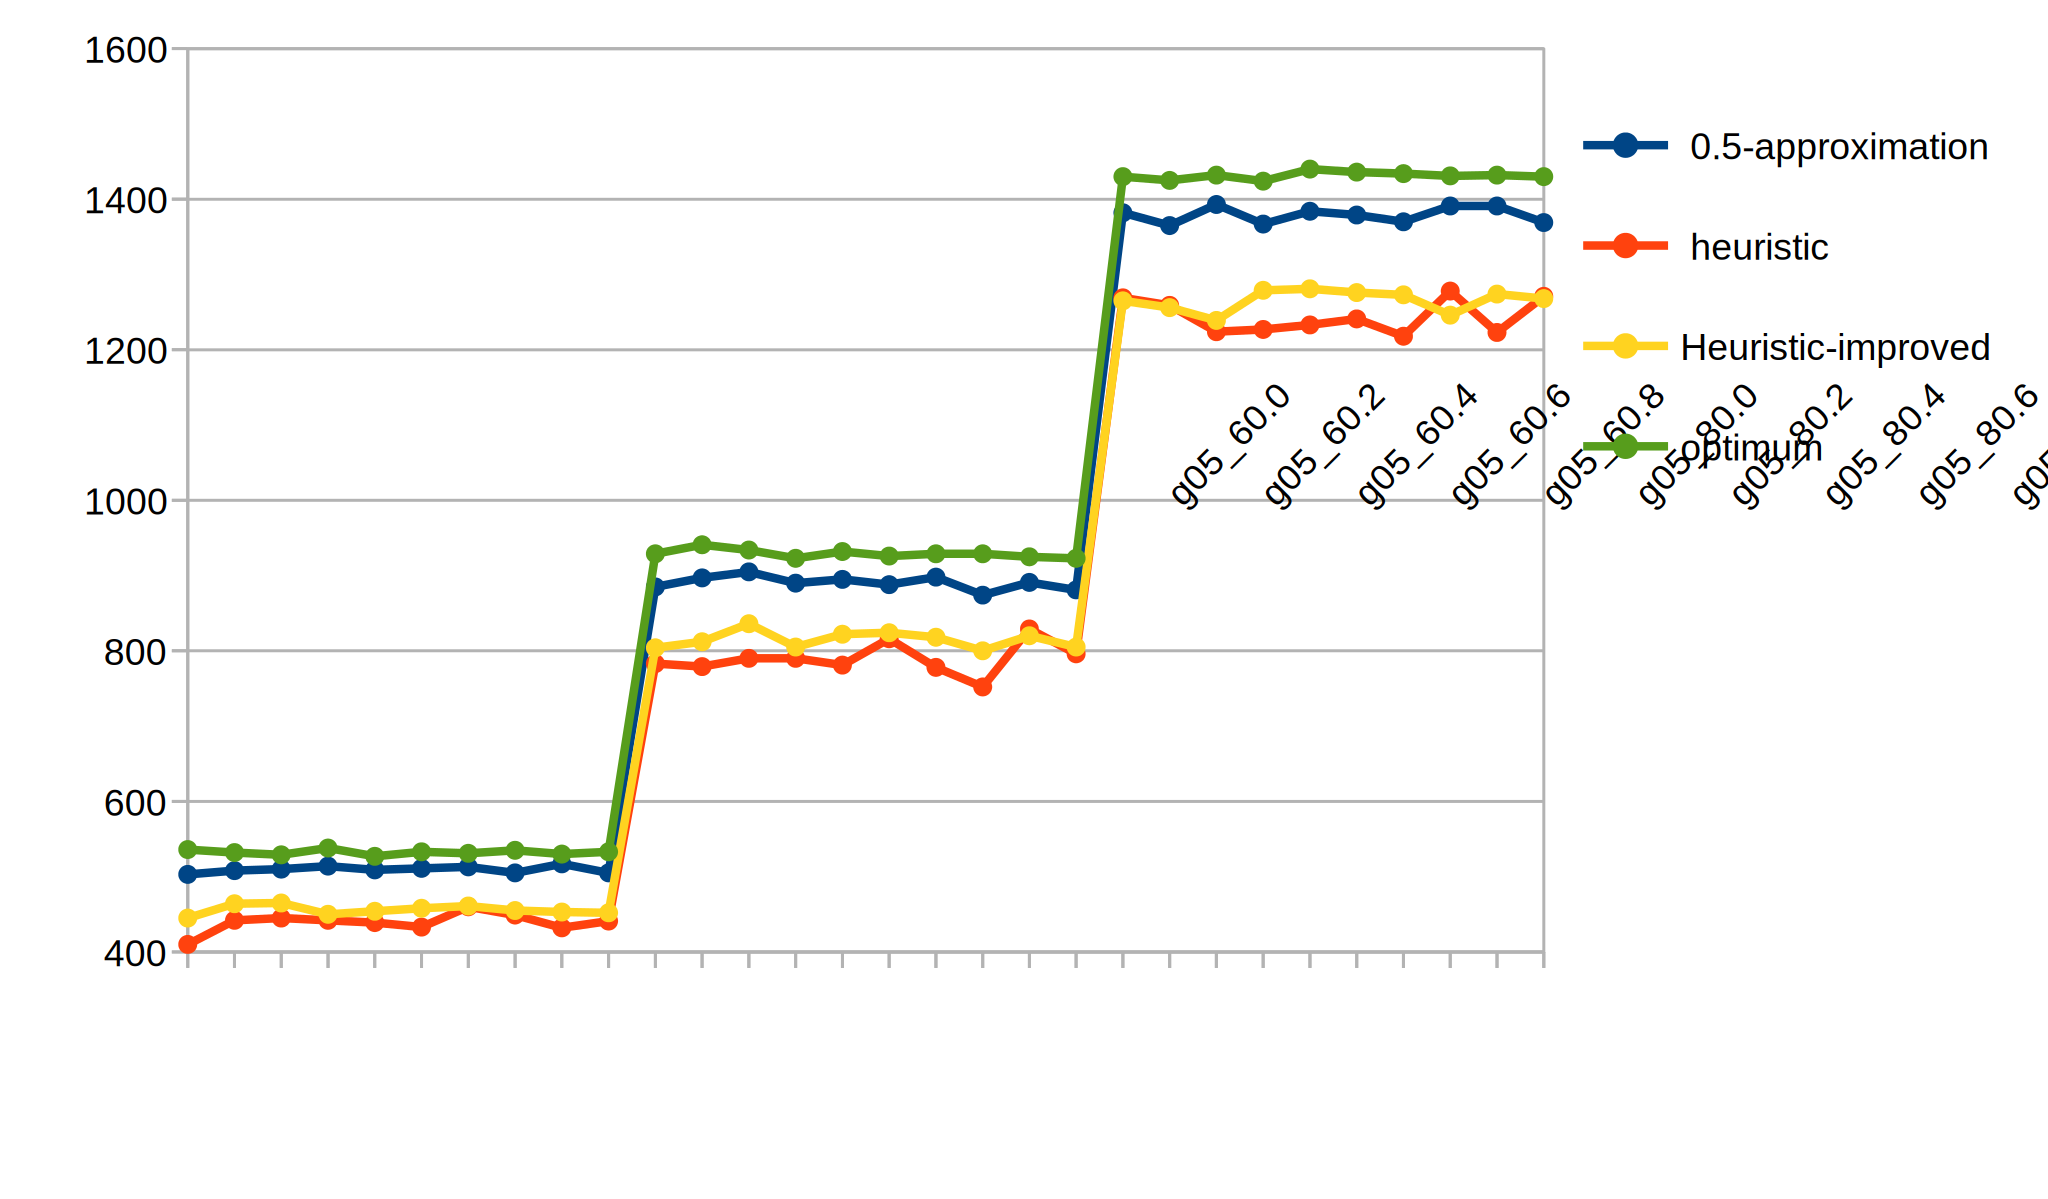
\includegraphics[height=0.4\textheight]{figures/solution_size.png}
  \end{center}
  \caption{Size of the results compared to the optimum (edges marks the total number of edges in the graph)}
  \label{fig:size}
\end{figure*}

\begin{figure*}
  \begin{center}
    \includesvg[width=1.05\textwidth]{figures/running_times}
  \end{center}
  \caption{Running times of every polynomial-time algorithm}
  \label{fig:run_time}
\end{figure*}



\section{Discussion and Conclusion}
% In this section, the results are discussed and interpreted. Finally, the work is summarized shortly.

In this work, I compared a basic heuristic and approximation algorithm and an ILP-formulation 
for exact computation of the max-cut problem.
For the heuristic and approximation we looked into methods of possibly improving their run time.
We showed that the basic implementation of the heuristic always is the fastest but gets beaten
by the approximation algorithm in terms of quality of the result. It might be surprising, that
the parallel heuristic is slower than the basic implementation.
But after considering the amount of work which is parallelised is quite small it becomes quite
clear, that the time saved by parallelising is negated by the amount of work necessary for
merging the results of the individual threads.
For this reason it might be better to use parallelism to generate multiple heuristics for
achieving better overall results. 

Another interesting observation is the better result quality of the approximation algorithm
compared to the heuristic.
The reason for this observation, are the guarantees we can make about the results.
As shown in Section \ref{sct:pre_approx} the approximation algorithm guarantees that the
result size is at least $\frac{1}{2}|E|$ where as the heuristic only produces results
with size $\frac{1}{2}|E|$ in expectation. This means the heuristic may produce results
which are smaller in size than the expectation.

For computing exact solutions with an ILP-solver it seems like density is the main factor
for increase in running time. This becomes especially clear, if we look at the running time
of the instance 'vc-exact\_027.gr' and 'g05\_60.0'.

\section{References}

\bibliographystyle{abbrvnat}
\bibliography{refs}

\end{document}
